\documentclass{article}

% NeurIPS High School Projects 2024 style. The HS track is non-anonymous, so we
% use the [preprint] option (shows authors; footer reads "Preprint. Work in progress.").
\usepackage[preprint]{neurips_2024}

\usepackage[utf8]{inputenc}
\usepackage[T1]{fontenc}
\usepackage{hyperref}
\usepackage{url}
\usepackage{booktabs}
\usepackage{amsmath}
\usepackage{amssymb}
\usepackage{amsfonts}
\usepackage{nicefrac}
\usepackage{microtype}
\usepackage{xcolor}
\usepackage{graphicx}
\usepackage{subcaption}
\usepackage{siunitx}
\usepackage{enumitem}
\usepackage[labelfont=bf,labelsep=period]{caption}

\graphicspath{{figures/}}

\title{Mapping the Invisible: Spatially Honest Evaluation and Environmental-Justice Auditing for Hyperlocal PM\textsubscript{2.5} Prediction}

\author{%
  Saketh Chebrolu \\
  St.~Mark's School of Texas \\
  Dallas, TX, USA \\
  \texttt{chebrolusaketh@gmail.com} \\
  \And
  Nathan Tan \\
  St.~Mark's School of Texas \\
  Dallas, TX, USA \\
  \texttt{nathantan2027@gmail.com} \\
}

\begin{document}
\maketitle

\begin{abstract}
Fine particulate matter (PM\textsubscript{2.5}) is the world's largest environmental cause of premature death, but regulatory monitors are far too sparse to see it at the neighborhood scale where exposure actually varies. Machine learning is widely used to fill that gap, yet two problems recur: models are evaluated with random train/test splits that quietly leak location-specific information, and their errors are almost never checked for fairness. We build a benchmark of 61{,}224 daily measurements from 240 low-cost sensors across four Texas metros and evaluate six regressors under \emph{leave-one-sensor-out} cross-validation (LOSO-CV), which forces a model to predict at locations it never saw. Random splits overstate accuracy by $\Delta R^2 \approx 0.22$ for the strongest models; an unweighted tree ensemble that scores $R^2{=}0.810$ on a random split drops to a pooled LOSO $R^2{=}0.753$. Auditing the same sensors against the EPA EJScreen environmental-justice index, observed PM\textsubscript{2.5} rises sharply with disadvantage ($r{=}0.760$, $p{<}10^{-45}$): \SI{77.2}{\percent} of highest-burden sites exceed the 2024 annual standard versus \SI{0.0}{\percent} of lowest-burden sites, a $5.6~\mu$g/m\textsuperscript{3} gap. Prediction bias stays near zero across every burden quartile ($\le\!0.12~\mu$g/m\textsuperscript{3}), so the disparity reflects the physical environment, not the model. We deploy these methods in a free public tool that maps daily PM\textsubscript{2.5} for all $\sim$6{,}900 Texas census tracts.
\end{abstract}

\section{Introduction}

Airborne particles 2.5 micrometers or smaller (PM\textsubscript{2.5}) penetrate deep into the lungs and bloodstream and are the single largest environmental risk factor for early death worldwide, contributing to an estimated seven million deaths a year and to heart, lung, and cognitive disease \citep{who2024ambient, pope2006health, landrigan2018lancet}. In 2024 the United States tightened its annual PM\textsubscript{2.5} standard to $9~\mu$g/m\textsuperscript{3} \citep{epa2024naaqs}, recognizing harm at concentrations once thought safe. The problem is that pollution changes block by block \citep{apte2017diesel, messier2018}, while reference monitors are scarce: Texas has roughly 30 million residents and fewer than 100 regulatory PM\textsubscript{2.5} stations. Dense networks of low-cost sensors paired with machine learning are the standard way to estimate pollution where no monitor exists \citep{ghahremanloo2021, zhang2024unmasking}.

Two issues undermine this literature, and both matter most for the communities that need accurate estimates the most. First, \textbf{evaluation is usually spatially dishonest}: a random train/test split puts some days from every sensor in both halves, letting a model memorize each site's quirks and report $R^2$ above 0.9, even though the real task---predicting where there is \emph{no} sensor---is exactly what such a split cannot measure \citep{roberts2017cross, meyer2019importance}. Second, \textbf{model error is rarely audited for equity}: if predictions are worse, or biased, in disadvantaged neighborhoods, an exposure map will understate risk precisely where it is greatest. We address both, and turn the result into a working public tool. Our contributions are:
\begin{itemize}[leftmargin=1.4em, itemsep=0.1em, topsep=0.2em]
\item \textbf{An honest benchmark.} On 61{,}224 sensor-days from 240 Texas sensors we run exhaustive leave-one-sensor-out cross-validation for six regressors and quantify how much random splitting inflates reported accuracy ($\Delta R^2 \approx 0.22$ for gradient-boosted trees).
\item \textbf{An environmental-justice audit.} We measure how observed PM\textsubscript{2.5} tracks the EPA EJScreen burden index ($r{=}0.760$) and show that the model's \emph{error} is unbiased across burden quartiles, so the disparity is not an artifact of where the model is accurate.
\item \textbf{A deployed tool.} We operationalize the method in a statewide production model and a free public map that serves daily tract-level PM\textsubscript{2.5} for all of urban Texas.
\end{itemize}

\section{Data and Methods}
\label{sec:methods}

\paragraph{Benchmark dataset.} We use 240 PurpleAir low-cost sensors across four Texas metros (Austin, $n{=}55$; Dallas--Fort Worth, $n{=}66$; Houston, $n{=}73$; San Antonio, $n{=}46$) over calendar year 2025, giving 61{,}224 daily records across 201 census tracts (mean PM\textsubscript{2.5} $6.98~\mu$g/m\textsuperscript{3}, median $5.68$). Readings use the EPA Barkjohn low-cost-sensor correction \citep{barkjohn2021} and are averaged to daily means. Each record carries 19 features in five groups: meteorology from the nearest NOAA GHCN station \citep{menne2012ghcn} (temperature, humidity, pressure); calendar terms (month, day-of-week, day-of-year); three within-sensor autoregressive terms (1- and 7-day lags and a 7-day rolling mean, shifted to prevent leakage); eight EPA EJScreen 2023 indicators joined by census-tract GEOID \citep{epa2022ejscreen}; and latitude/longitude.

\paragraph{Models.} We compare multiple linear regression (MLR), an RBF support-vector regressor (SVR), random forest (RF), LightGBM, XGBoost, and an unweighted mean of the three tree models (Ensemble), our deployment estimator. Hyperparameters follow common defaults from the air-quality literature \citep{ghahremanloo2021, zhang2024unmasking}; all seeds are fixed.

\paragraph{Spatially honest evaluation.} Under leave-one-sensor-out cross-validation we remove one sensor entirely, train on the remaining sensors, and predict the held-out sensor's days; repeating over all sensors yields an unbiased estimate of accuracy at an unmonitored location. We contrast this with a random 80/20 split, whose gap to LOSO-CV measures how much location-specific leakage inflates a score. SVR's $\mathcal{O}(n^2)$ kernel cost makes 240 refits intractable, so it is reported on the random split only.

\paragraph{Deployed production model.} The public tool is powered by a stronger successor trained on the same principles. It is a four-model ensemble (adding CatBoost) over 38 features that extend the benchmark set with the dominant signal for spatial extrapolation---the same-day mean PM\textsubscript{2.5} of neighboring sensors at 25, 50, and 100~km---plus NOAA Hazard Mapping System smoke and Copernicus satellite aerosol optical depth. It is trained on 285{,}798 sensor-days from 310 sensors spanning 55 Texas counties (January 2021--May 2026). Because the neighbor features could leak a held-out sensor's own value, we recompute them inside every fold with that sensor removed; the resulting leakage-free LOSO $R^2$ is $0.714$ (random-split $0.839$).

\section{Results}
\label{sec:results}

\subsection{Honest evaluation cuts reported accuracy by a fifth}
Table~\ref{tab:bench} shows the central methodological finding. On a random split, gradient-boosted trees look excellent ($R^2$ of 0.83--0.84). Under leave-one-sensor-out evaluation the \emph{same models} fall to per-fold $R^2$ near 0.61, a drop of $\Delta R^2$ of 0.21 (LightGBM) and 0.23 (XGBoost), and at least 0.20 for every nonlinear model. Linear regression, which cannot memorize local quirks, still loses ground (random $0.588 \rightarrow$ LOSO $0.249$), confirming that the leaked signal is spread across many features rather than a single one. The unweighted ensemble is the most stable estimator across sensors (the smallest spread of per-fold $R^2$, $\sigma{=}0.30$ versus 0.42--0.44 for the single boosters); pooled over all 61{,}221 held-out sensor-days it reaches $R^2{=}0.753$ with RMSE $2.70~\mu$g/m\textsuperscript{3}. The lesson is concrete: a study reporting only the random-split number would advertise ``excellent'' ($R^2{>}0.83$) accuracy for a tool that, where it is actually needed, performs closer to $R^2 \approx 0.75$.

\begin{table}[t]
\caption{Random 80/20 split vs.\ leave-one-sensor-out cross-validation (LOSO-CV) on 61{,}224 sensor-days from 240 Texas sensors. LOSO entries are means over 239 folds (one sensor lacked enough held-out days to score). $\Delta R^2$ is the random-split over-estimate. SVR is omitted from LOSO-CV for cost. Best honest (LOSO) $R^2$ in bold.}
\label{tab:bench}
\centering
\small
\setlength{\tabcolsep}{6pt}
\begin{tabular}{lccccc}
\toprule
& \multicolumn{2}{c}{\textbf{Random 80/20}} & \multicolumn{2}{c}{\textbf{LOSO-CV (239 folds)}} & \\
\cmidrule(lr){2-3}\cmidrule(lr){4-5}
\textbf{Model} & $R^2$ & RMSE & $R^2$ & RMSE & $\Delta R^2$ \\
\midrule
MLR       & 0.588 & 3.61 & 0.249 & 3.26 & 0.339 \\
SVR       & 0.479 & 4.06 & ---   & ---  & ---   \\
RF        & 0.717 & 2.99 & 0.468 & 2.70 & 0.249 \\
LightGBM  & 0.827 & 2.34 & \textbf{0.621} & 2.21 & 0.206 \\
XGBoost   & 0.836 & 2.28 & 0.610 & 2.21 & 0.226 \\
Ensemble  & 0.810 & 2.45 & 0.608 & 2.29 & 0.202 \\
\bottomrule
\end{tabular}
\end{table}

\subsection{The pollution--disadvantage gradient is steep}
Figure~\ref{fig:ej} audits the 239 sensor sites against the EJScreen environmental-justice index, a Texas-percentile composite of demographic and pollution-burden indicators. Annual-mean observed PM\textsubscript{2.5} rises strongly with disadvantage ($r{=}0.760$, $p{<}10^{-45}$). Splitting the sites into burden quartiles makes the consequence stark: \SI{0.0}{\percent} of the lowest-burden quartile (Q1) exceed the 2024 annual standard of $9~\mu$g/m\textsuperscript{3}, against \SI{1.7}{\percent} (Q2), \SI{38.7}{\percent} (Q3), and \SI{77.2}{\percent} of the highest-burden quartile (Q4). Mean exposure climbs from $4.65~\mu$g/m\textsuperscript{3} in Q1 to $10.26$ in Q4---a $5.6~\mu$g/m\textsuperscript{3} gap measured directly from the sensors, with no model in the loop. This mirrors national findings \citep{tessum2021pm25, jbaily2022air, colmer2020disparities} but at neighborhood resolution within a single state.

\begin{figure}[t]
  \centering
  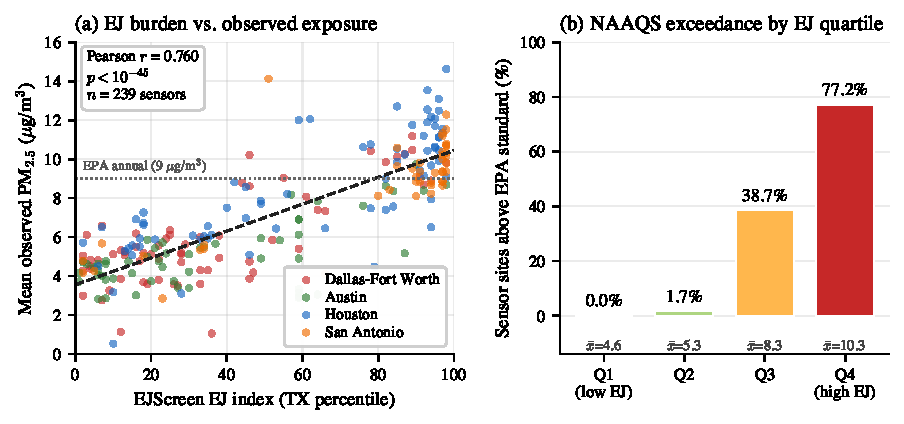
\includegraphics[width=\linewidth]{fig_ej.pdf}
  \caption{Environmental-justice audit over 239 sensor sites. (a) Observed annual-mean PM\textsubscript{2.5} versus the EJScreen burden index, colored by metro ($r{=}0.760$). (b) Share of sites exceeding the 2024 annual standard, by burden quartile; $\bar{x}$ is each quartile's mean PM\textsubscript{2.5} ($\mu$g/m\textsuperscript{3}).}
  \label{fig:ej}
\end{figure}

\subsection{Is the gradient just where the model is worse? No.}
A fairness audit is only meaningful if the model's mistakes are not themselves concentrated in disadvantaged areas. Figure~\ref{fig:fair} stratifies per-sensor LOSO error by burden quartile. Signed bias stays within $\pm 0.12~\mu$g/m\textsuperscript{3} of zero in every quartile, so the model does not systematically under- or over-state exposure where burden is highest---the key precondition for using its predictions in equity analysis. Absolute error does grow with burden (RMSE rising from $1.51~\mu$g/m\textsuperscript{3} in Q1 to $2.96$ in Q4), but this tracks the higher mean and variance of pollution in those areas rather than directional bias; users of the deployed map should read predictions in high-burden areas as unbiased but wider in uncertainty. Because the exposure gradient in Figure~\ref{fig:ej} comes from observed readings and the model's bias is flat, the disparity is a property of Texas air quality, not of the estimator.

\begin{figure}[t]
  \centering
  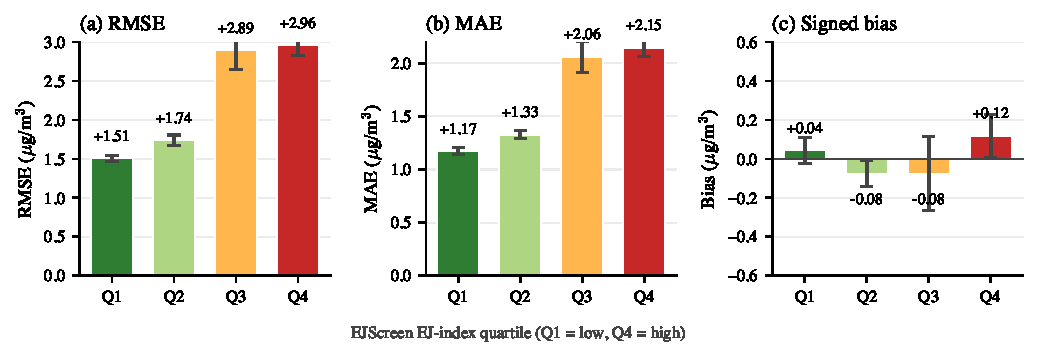
\includegraphics[width=\linewidth]{fig_fairness.pdf}
  \caption{Per-sensor LOSO error by EJ burden quartile. (a) RMSE and (b) MAE rise with burden, following higher pollution levels; (c) signed bias is near zero throughout, so the model adds no directional error in disadvantaged areas. Bars show mean $\pm$ one standard error across sensors.}
  \label{fig:fair}
\end{figure}

\section{Deployment and Social Impact}
\label{sec:deploy}

These methods run a free, public web tool (\url{https://sharedskiesinitiative.org/real-time-map}) that predicts daily PM\textsubscript{2.5} for all $\sim$6{,}900 Texas census tracts and refreshes from the live sensor network, with no login or cost. The same-day neighbor, satellite-smoke, and aerosol features let the production model track wildfire and dust events that static models miss, and the leakage-free LOSO $R^2$ of $0.714$ is an honest estimate of its accuracy at an unmonitored tract---the number that matters for the people relying on it. The intent is direct: give residents of the 30 million-person state, and especially the high-burden communities identified above, a trustworthy neighborhood-scale view of air they cannot see, so that individuals can limit exposure on bad days and advocates and agencies can target monitoring and mitigation where the data show it is most needed.

\section{Limitations}
\label{sec:limits}

The benchmark spans one calendar year, so performance under unusual regimes (a once-in-a-decade smoke event) is untested. Low-cost sensors carry residual humidity bias even after correction \citep{barkjohn2021}, so absolute levels may inherit a network-wide offset. EJScreen indicators are updated infrequently and are treated as fixed over the study window. Finally, even under honest evaluation, $R^2 \approx 0.75$ leaves real variance unexplained by meteorological, temporal, and contextual features; satellite aerosol depth and atmospheric-transport inputs are promising next additions.

\section{Conclusion}
\label{sec:conclusion}

Evaluating PM\textsubscript{2.5} models the way they are deployed---predicting at locations without sensors---lowers reported accuracy by about $\Delta R^2{=}0.22$ for the best models, a correction the field should adopt to avoid over-promising. Within that honest frame, a low-cost sensor network reveals a steep pollution--disadvantage gradient ($r{=}0.760$; \SI{77.2}{\percent} vs.\ \SI{0.0}{\percent} exceedance between the highest- and lowest-burden quartiles) that the model's own near-zero bias confirms is real, not an artifact. We turn the analysis into a free statewide tool so the communities most exposed can finally see, and act on, the air around them.

\begin{ack}
This work received no external funding. The authors declare no competing financial or non-financial interests. The public tool is operated on a non-commercial basis. We thank the PurpleAir community for open sensor data and the U.S.\ EPA and NOAA for open environmental data.
\end{ack}

\small
\bibliographystyle{plainnat}
\bibliography{references}

\end{document}
